% =============================================================================
% ENGINEERING DESIGN: 3-NODE PSI-TIMING NETWORK DEMONSTRATOR
% Supporting document for Patent #5
% Author: Gary Thomas Alcock
% =============================================================================

\documentclass[12pt,letterpaper]{article}

\usepackage{amsmath,amssymb}
\usepackage{graphicx}
\usepackage{siunitx}
\usepackage{booktabs}
\usepackage{hyperref}
\usepackage{geometry}
\usepackage{tikz}
\usetikzlibrary{arrows.meta,positioning,decorations.pathmorphing,calc}
\usepackage{enumitem}
\usepackage{fancyhdr}
\usepackage{longtable}

\geometry{margin=1in}
\pagestyle{fancy}
\fancyhead[L]{3-Node $\psi$-Timing Network Demonstrator}
\fancyhead[R]{Engineering Design Document}
\fancyfoot[C]{\thepage}

\title{Engineering Design Document:\\
Three-Node $\psi$-Timing Network Demonstrator\\[10pt]
\large Supporting Patent \#5: $\psi$-Field Geometry-Locked Navigation,
Timing, and Communications}
\author{Gary Thomas Alcock\\
Density Field Dynamics Research}
\date{\today}

\begin{document}
\maketitle
\tableofcontents
\newpage

% =============================================================================
\section{Executive Summary}
% =============================================================================

This document presents the complete engineering design for a three-node
$\psi$-field timing network demonstrator. The system demonstrates the
core claims of Patent \#5: geometry-locked navigation, sub-femtosecond
timing without GNSS, and intrinsic anti-spoofing through $\psi$-curvature
verification.

The demonstrator consists of three nodes arranged in an equilateral
triangle with 10-meter baselines. Each node contains an ultra-stable
optical oscillator, a phase-coherent fiber link, a high-resolution
phasemeter, and a gravity gradient sensor. The nodes exchange
phase-coherent optical signals through stabilized fibers, enabling
differential $\psi$-phase measurement at the $10^{-18}$ level and
timing synchronization at the sub-femtosecond level.

\paragraph{Key specifications:}
\begin{itemize}[nosep]
\item Baseline: 10~m equilateral triangle
\item $\psi$-phase precision: $< 10^{-18}$ at 1~s averaging
\item Position accuracy: $< 0.1$~mm at 1~s
\item Timing precision: $< 0.3$~fs at 1~s, $< 10$~as at 1000~s
\item Anti-spoofing threshold: 10~m (1~E gradiometer)
\item Total estimated cost: \$2--5M (leveraging existing laboratory infrastructure)
\end{itemize}

% =============================================================================
\section{System Architecture}
% =============================================================================

\subsection{Network Topology}

The demonstrator consists of three identical nodes (N1, N2, N3) arranged at
the vertices of an equilateral triangle with side length $L = 10$~m. A
mobile test receiver (R) operates within the triangle for position
verification.

\begin{figure}[h]
\centering
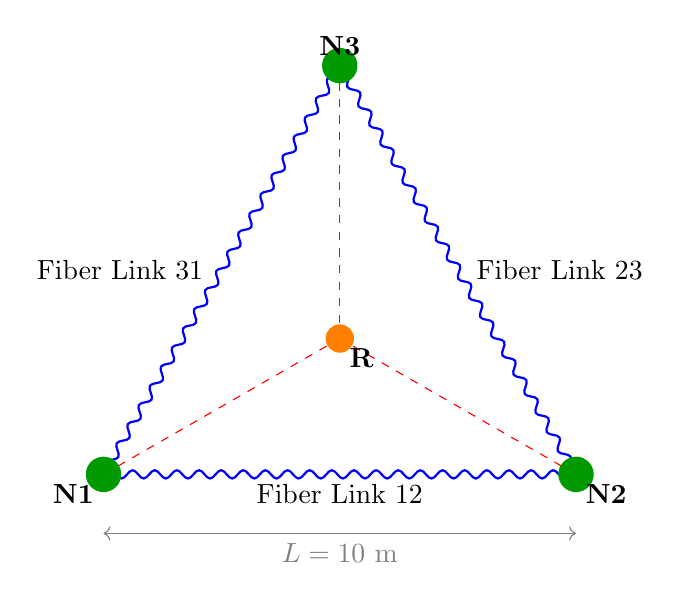
\begin{tikzpicture}[scale=1.5]
  % Triangle vertices
  \coordinate (N1) at (0,0);
  \coordinate (N2) at (4,0);
  \coordinate (N3) at (2,3.46);
  \coordinate (R) at (2,1.15);

  % Fiber links
  \draw[blue,thick,decorate,decoration={snake,amplitude=1.5pt,segment length=8pt}]
    (N1) -- (N2) node[midway,below,black] {Fiber Link 12};
  \draw[blue,thick,decorate,decoration={snake,amplitude=1.5pt,segment length=8pt}]
    (N2) -- (N3) node[midway,right,black,xshift=3pt] {Fiber Link 23};
  \draw[blue,thick,decorate,decoration={snake,amplitude=1.5pt,segment length=8pt}]
    (N3) -- (N1) node[midway,left,black,xshift=-3pt] {Fiber Link 31};

  % psi-field lines to receiver
  \draw[red,dashed,->] (N1) -- (R);
  \draw[red,dashed,->] (N2) -- (R);
  \draw[red,dashed,->] (N3) -- (R);

  % Nodes
  \fill[green!60!black] (N1) circle (0.15) node[below left,black] {\textbf{N1}};
  \fill[green!60!black] (N2) circle (0.15) node[below right,black] {\textbf{N2}};
  \fill[green!60!black] (N3) circle (0.15) node[above,black] {\textbf{N3}};

  % Receiver
  \fill[orange] (R) circle (0.12) node[below right,black] {\textbf{R}};

  % Dimensions
  \draw[<->,gray] (0,-0.5) -- (4,-0.5) node[midway,below] {$L = 10$~m};
\end{tikzpicture}
\caption{Network topology: three fixed nodes (N1--N3) connected by
stabilized fiber links, with mobile receiver R. Red dashed lines indicate
$\psi$-field measurement paths.}
\label{fig:topology}
\end{figure}

\subsection{Functional Block Diagram}

Each node implements the following functional blocks:

\begin{figure}[h]
\centering
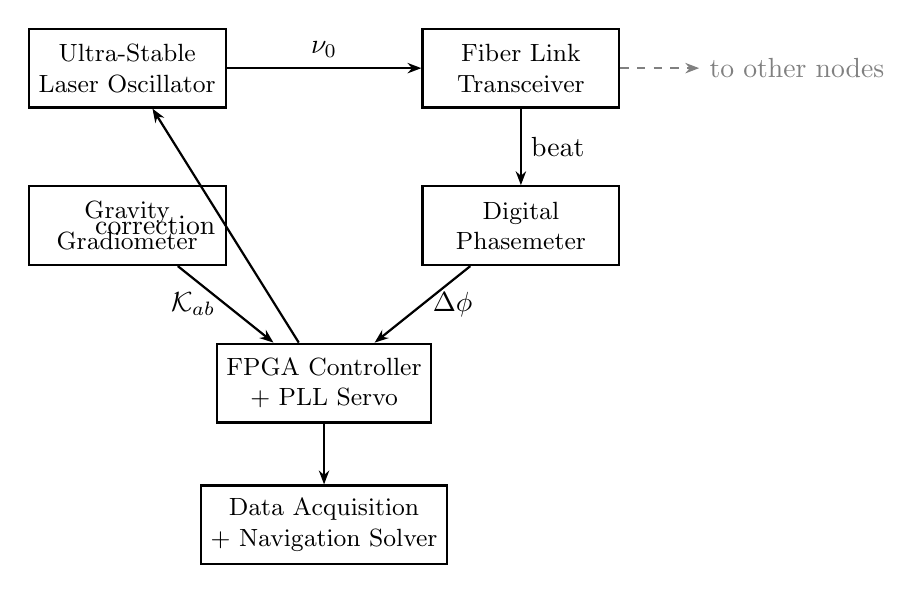
\begin{tikzpicture}[
  block/.style={draw, thick, minimum width=2.5cm, minimum height=1cm,
    align=center, font=\small},
  arrow/.style={-{Stealth[length=5pt]}, thick}
]
  % Blocks
  \node[block] (osc) at (0,4) {Ultra-Stable\\Laser Oscillator};
  \node[block] (fiber) at (5,4) {Fiber Link\\Transceiver};
  \node[block] (phase) at (5,2) {Digital\\Phasemeter};
  \node[block] (grad) at (0,2) {Gravity\\Gradiometer};
  \node[block] (fpga) at (2.5,0) {FPGA Controller\\+ PLL Servo};
  \node[block] (data) at (2.5,-1.8) {Data Acquisition\\+ Navigation Solver};

  % Arrows
  \draw[arrow] (osc) -- (fiber) node[midway,above] {$\nu_0$};
  \draw[arrow] (fiber) -- (phase) node[midway,right] {beat};
  \draw[arrow] (phase) -- (fpga) node[midway,right] {$\Delta\phi$};
  \draw[arrow] (grad) -- (fpga) node[midway,left] {$\mathcal{K}_{ab}$};
  \draw[arrow] (fpga) -- (osc) node[midway,left] {correction};
  \draw[arrow] (fpga) -- (data);
  \draw[arrow,dashed,gray] (fiber.east) -- ++(1,0) node[right] {to other nodes};
\end{tikzpicture}
\caption{Functional block diagram of a single node.}
\label{fig:block}
\end{figure}

% =============================================================================
\section{Subsystem Specifications}
% =============================================================================

\subsection{Ultra-Stable Laser Oscillator}

\begin{table}[h]
\centering
\caption{Laser oscillator specifications.}
\label{tab:laser}
\begin{tabular}{@{}lll@{}}
\toprule
Parameter & Specification & Notes \\
\midrule
Wavelength & 1542 nm (or 698 nm) & Telecom-compatible / Sr clock \\
Linewidth & $< 10$~mHz & Cavity-stabilized \\
Frequency stability & $\sigma_y < 4\times10^{-17}$ at 1~s & ULE cavity reference \\
Drift rate & $< 10$~mHz/s & Thermal compensation \\
Output power & $> 10$~mW & Sufficient for 10-m fiber links \\
Cavity finesse & $> 300{,}000$ & Standard ULE/Zerodur \\
Cavity length & 10 cm & Spacer material: ULE glass \\
Temperature control & $\pm 1$~mK & Active thermal stabilization \\
Vibration isolation & $< 10^{-7}$~g/$\sqrt{\text{Hz}}$ at 1 Hz & Passive + active platform \\
\bottomrule
\end{tabular}
\end{table}

\paragraph{Implementation options:}
\begin{enumerate}
\item \textbf{Preferred:} Cavity-stabilized laser at 1542~nm locked to a
silicon single-crystal cavity at 124~K (cryogenic silicon cavity). This
achieves $\sigma_y \sim 4\times10^{-17}$ at 1~s with thermal noise floor
at $\sim 10^{-17}$~\cite{Matei2017}.

\item \textbf{Alternative:} ULE cavity at room temperature with dual-layer
thermal shielding. Achieves $\sigma_y \sim 10^{-16}$ at 1~s, sufficient for
initial demonstrations.

\item \textbf{Advanced:} Lock to an optical lattice clock (Sr or Yb) for
ultimate accuracy at $10^{-18}$ level. This upgrades the demonstrator from
a timing system to a full $\psi$-field measurement system.
\end{enumerate}

\subsection{Fiber Link Transceiver}

\begin{table}[h]
\centering
\caption{Fiber link specifications.}
\label{tab:fiber}
\begin{tabular}{@{}lll@{}}
\toprule
Parameter & Specification & Notes \\
\midrule
Fiber type & Single-mode (SMF-28) & Low loss at 1542~nm \\
Link length & 10--15~m (incl.\ routing) & Through conduit \\
Doppler cancellation & Active, $< 10^{-19}$ at 1~s & AOM-based round-trip \\
AOM frequency & 80~MHz & Standard double-pass \\
Beat detection bandwidth & 100~kHz & Sufficient for servo \\
Optical power at detector & $> 100$~$\mu$W & After fiber losses \\
Connector type & FC/APC & Low back-reflection \\
Fiber noise suppression & $> 60$~dB at 1~Hz & Active noise cancellation \\
\bottomrule
\end{tabular}
\end{table}

\paragraph{Doppler cancellation scheme:}
The standard technique for fiber noise cancellation uses an acousto-optic
modulator (AOM) at the local end and a Faraday mirror at the remote end.
The round-trip phase is detected and used to servo the AOM frequency,
canceling fiber phase noise. For a 10-m fiber, the residual noise after
cancellation is dominated by the servo bandwidth, typically achieving
$\sigma_y < 10^{-19}$ at 1~s for fiber lengths $< 100$~m.

The key observable is the beat frequency between the local oscillator and the
round-trip-corrected signal from the remote node:
\begin{equation}
\nu_{\rm beat} = \nu_A - \nu_B + \delta\nu_{\rm Doppler}^{\rm residual}
+ \delta\nu_{\rm grav},
\end{equation}
where $\delta\nu_{\rm grav} = \nu_0\,(\psi_A - \psi_B)/2$ is the
gravitational frequency difference encoding the $\psi$-phase information.

\subsection{Digital Phasemeter}

\begin{table}[h]
\centering
\caption{Phasemeter specifications.}
\label{tab:phasemeter}
\begin{tabular}{@{}lll@{}}
\toprule
Parameter & Specification & Notes \\
\midrule
Input bandwidth & DC -- 100~kHz & Covers servo bandwidth \\
ADC resolution & 16~bit & At 1~MHz sample rate \\
Phase precision & $< 1$~$\mu$rad at 1~s & $\sim 10^{-19}$ fractional \\
Dynamic range & $> 120$~dB & For varying signal levels \\
Channels & 6 (two per link) & 3 links, bidirectional \\
Latency & $< 10$~$\mu$s & For real-time servo \\
Data output & Ethernet + PPS trigger & GPS-disciplined PPS optional \\
\bottomrule
\end{tabular}
\end{table}

\paragraph{Architecture:}
The phasemeter uses a digital IQ demodulation scheme:
\begin{enumerate}
\item The beat signal is digitized at 1~MHz (16-bit ADC).
\item A numerically controlled oscillator (NCO) generates the reference.
\item IQ multiplication and low-pass filtering extract the phase.
\item Phase unwrapping maintains continuous phase tracking.
\end{enumerate}

The phase measurement is related to the $\psi$-phase observable by
\begin{equation}
\phi_{\rm meas}(t) = 2\pi\int_0^t \nu_{\rm beat}(t')\,dt'
= 2\pi\nu_0\int_0^t \frac{\psi_A(t') - \psi_B(t')}{2}\,dt'
+ \text{oscillator terms}.
\end{equation}

\subsection{Gravity Gradiometer}

\begin{table}[h]
\centering
\caption{Gradiometer specifications.}
\label{tab:gradiometer}
\begin{tabular}{@{}lll@{}}
\toprule
Parameter & Specification & Notes \\
\midrule
Sensitivity & $< 1$~E/$\sqrt{\text{Hz}}$ & 1~E $= 10^{-9}$~s$^{-2}$ \\
Bandwidth & 0.01--1~Hz & Adequate for static + tidal \\
Measurement axes & Full tensor (5 independent) & Dual-axis + cross-terms \\
Integration time & 100~s for 0.1~E precision & \\
Operating temperature & Room temperature (300~K) & \\
Size & $< 50 \times 50 \times 50$~cm & Per axis \\
\bottomrule
\end{tabular}
\end{table}

\paragraph{Implementation options:}
\begin{enumerate}
\item \textbf{Atom interferometer gradiometer:} Cold-atom clouds in free
fall, interrogated by Raman pulses. Achieves $\sim$1--10~mE/$\sqrt{\rm Hz}$.
Current state of the art for portable devices.

\item \textbf{Superconducting gradiometer:} Paired superconducting
accelerometers with matched response. Achieves $\sim$0.1~E/$\sqrt{\rm Hz}$
but requires cryogenics.

\item \textbf{MEMS differential accelerometer:} Paired high-sensitivity
MEMS devices. Lower sensitivity ($\sim$10~E/$\sqrt{\rm Hz}$) but much
lower cost and complexity. Suitable for initial proof-of-concept.
\end{enumerate}

For the demonstrator, a MEMS-based approach is recommended for Phase~1--3
(cost-effective, proves the concept), with upgrade path to atom
interferometry for Phase~4--5 (higher sensitivity for anti-spoofing tests).

\subsection{FPGA Controller}

\begin{table}[h]
\centering
\caption{Controller specifications.}
\label{tab:controller}
\begin{tabular}{@{}lll@{}}
\toprule
Parameter & Specification & Notes \\
\midrule
FPGA & Xilinx Zynq 7020 (or equivalent) & ARM + FPGA fabric \\
Clock & $< 1$~ps jitter & OCXO-disciplined \\
DAC resolution & 20~bit & For oscillator tuning \\
DAC update rate & 1~MHz & Matches ADC \\
Servo bandwidth & 1--100~Hz (configurable) & PI controller \\
Network interface & 1~GbE & Node-to-node communication \\
PPS output & $< 100$~ps accuracy & For external synchronization \\
Power & $< 20$~W per node & Standard lab power supply \\
\bottomrule
\end{tabular}
\end{table}

\paragraph{Servo algorithm:}
The FPGA implements a digital PI controller:
\begin{equation}
u(n) = K_p\,e(n) + K_i\,T_s\sum_{k=0}^{n} e(k),
\end{equation}
where $e(n) = \phi_{\rm ref}(n) - \phi_{\rm meas}(n)$ is the phase error
at sample $n$, $T_s$ is the sample period, and $K_p$, $K_i$ are the
proportional and integral gains.

The servo output drives a voltage-controlled oscillator (VCO) or AOM
frequency to steer the local oscillator phase. The closed-loop bandwidth is
set by the desired noise performance:
\begin{itemize}
\item Narrow bandwidth ($B_L \sim 1$~Hz): Lowest noise floor, but slow
response to perturbations. Suitable for static nodes.
\item Wide bandwidth ($B_L \sim 100$~Hz): Fast tracking, higher noise floor.
Suitable for the mobile receiver.
\end{itemize}

% =============================================================================
\section{$\psi$-Phase Measurement and Calibration}
% =============================================================================

\subsection{Measurement Principle}

The fundamental measurement is the differential gravitational frequency
shift between two nodes connected by a stabilized fiber link. After
Doppler cancellation, the residual beat frequency encodes:
\begin{equation}
\Delta\nu_{AB}^{\rm residual} = \nu_0 \cdot \frac{\psi_A - \psi_B}{2}
+ \delta\nu_{\rm systematic},
\end{equation}
where $\delta\nu_{\rm systematic}$ includes:
\begin{itemize}
\item Residual fiber noise (after cancellation): $< 10^{-19}\nu_0$
\item Thermal drift of cavities: $\sim 10^{-16}\nu_0$/hr (correctable)
\item Barometric pressure effects: $\sim 10^{-17}\nu_0$/mbar
\item Tidal gravity variations: $\sim 3\times10^{-17}\nu_0$ (12.4-hr period)
\end{itemize}

\subsection{Height Difference Calibration}

For two nodes at the same horizontal position but different heights
$h_A$, $h_B$:
\begin{equation}
\psi_A - \psi_B = \frac{2g(h_A - h_B)}{c^2}.
\end{equation}
A 1-mm height difference produces:
\begin{equation}
\Delta\psi = \frac{2\times 9.8 \times 10^{-3}}{(3\times10^8)^2}
= 2.2\times10^{-19}.
\end{equation}
This is measurable with current optical clock technology at averaging
times of $\sim 100$~s, providing both a calibration reference and a
direct demonstration of $\psi$-field measurement.

\subsection{Systematic Error Budget}

\begin{table}[h]
\centering
\caption{Systematic error budget for differential $\psi$-phase measurement.}
\label{tab:systematics}
\begin{tabular}{@{}lcl@{}}
\toprule
Error source & Magnitude & Mitigation \\
\midrule
Height survey error ($\pm$0.1~mm) & $2\times10^{-20}$ & Precision leveling \\
Fiber chromatic dispersion & $< 10^{-21}$ & Single-frequency operation \\
Residual Doppler & $< 10^{-19}$ at 1~s & Active cancellation \\
Cavity thermal noise & $\sim 4\times10^{-17}$ at 1~s & Averages down as $\tau^{-1/2}$ \\
Barometric loading & $\sim 10^{-18}$/mbar & Pressure monitoring \\
Tidal variation & $\sim 3\times10^{-17}$ (known) & Model and subtract \\
Blackbody radiation shift & $\sim 10^{-18}$ & Temperature monitoring \\
AC Stark (stray light) & $< 10^{-19}$ & Light baffling \\
\midrule
\textbf{RSS systematic floor} & $\sim 5\times10^{-20}$ & After corrections \\
\bottomrule
\end{tabular}
\end{table}

% =============================================================================
\section{Navigation Solver}
% =============================================================================

\subsection{Algorithm}

The navigation solver takes as input the three differential $\psi$-phases
$\{\Delta\psi_{12}, \Delta\psi_{23}, \Delta\psi_{31}\}$ measured at the
receiver R, and outputs the receiver position $\mathbf{r}_R = (x_R, y_R, z_R)$
and clock bias $\delta t_R$.

\paragraph{Step 1: Linearization.}
For a uniform field ($\nabla\psi = 0$), the differential phase is
proportional to the range difference:
\begin{equation}
\Delta\psi_{ij} = \psi_0 (L_{iR} - L_{jR}).
\end{equation}
This defines a hyperboloid. Three hyperboloids (from three pairs) intersect
at the receiver position.

\paragraph{Step 2: Gauss--Newton iteration.}
Starting from an initial estimate $\hat{\mathbf{r}}_R^{(0)}$ (e.g., the
centroid of the triangle), iterate:
\begin{equation}
\hat{\mathbf{r}}_R^{(k+1)} = \hat{\mathbf{r}}_R^{(k)}
+ (\mathbf{J}^T\mathbf{W}\mathbf{J})^{-1}\mathbf{J}^T\mathbf{W}
\bigl(\Delta\boldsymbol{\psi}^{\rm meas}
- \Delta\boldsymbol{\psi}^{\rm pred}(\hat{\mathbf{r}}_R^{(k)})\bigr),
\end{equation}
where $\mathbf{J}$ is the $3\times3$ Jacobian matrix with elements
\begin{equation}
J_{(ij),a} = \frac{\partial\Delta\psi_{ij}}{\partial r_{R,a}}
= \psi_0\left(\frac{r_{R,a} - r_{i,a}}{L_{iR}}
- \frac{r_{R,a} - r_{j,a}}{L_{jR}}\right).
\end{equation}

\paragraph{Step 3: Convergence.}
For the 10-m triangle with the receiver near the centroid, convergence
to sub-millimeter accuracy typically requires 3--5 iterations from
any initial point within the triangle.

\subsection{Position Dilution of Precision}

For the equilateral triangle geometry with the receiver at the centroid,
the position dilution of precision (PDOP) is:
\begin{equation}
\text{PDOP} = \frac{2\sqrt{3}}{\psi_0\,L\,\text{SNR}_\psi}
= \frac{2\sqrt{3}}{10^{-9}\times 10\times \text{SNR}_\psi}.
\end{equation}
For $\text{SNR}_\psi = 10^9$ (corresponding to $\sigma_{\Delta\psi} = 10^{-18}$
with $\psi_0 \sim 10^{-9}$):
\begin{equation}
\text{PDOP} \approx \frac{3.5}{10^{-9}\times 10\times 10^9} = 0.35.
\end{equation}
The position error is then
$\sigma_r = \text{PDOP}\times c\,\sigma_t = 0.35\times 3\times10^8
\times 3\times10^{-16} \approx 3\times10^{-8}$~m $= 30$~nm, which is
at the level of seismic noise. The practical limit is set by the
oscillator noise floor rather than the geometry.

% =============================================================================
\section{Anti-Spoofing Verification}
% =============================================================================

\subsection{Test Procedure}

The anti-spoofing capability is verified by:
\begin{enumerate}
\item Establishing the baseline $\psi$-curvature map at all three
node positions using the gradiometer.
\item Introducing a known mass perturbation (e.g., 1000~kg of lead at a
known position) and observing the change in the gradiometer reading.
\item Computing the position solution with and without the mass perturbation.
\item Verifying that the curvature check (integrity monitor) correctly
flags the perturbation.
\end{enumerate}

\subsection{Mass Perturbation Calculation}

A point mass $M$ at distance $d$ from the gradiometer produces a
gravity gradient signal of order:
\begin{equation}
\Delta\Gamma \sim \frac{2GM}{d^3}.
\end{equation}
For $M = 1000$~kg at $d = 2$~m:
\begin{equation}
\Delta\Gamma = \frac{2\times 6.67\times10^{-11}\times 10^3}{8}
\approx 1.7\times10^{-8}\,\text{s}^{-2} = 17\,\text{E}.
\end{equation}
This is well above the 1~E detection threshold, providing a clear
demonstration of the anti-spoofing concept.

The corresponding $\psi$-curvature perturbation is:
\begin{equation}
\delta\mathcal{K} = \frac{2\Delta\Gamma}{c^2}
\approx 3.7\times10^{-25}\,\text{m}^{-2}.
\end{equation}

% =============================================================================
\section{Timing Performance Verification}
% =============================================================================

\subsection{Allan Deviation Measurement}

The primary timing metric is the modified Allan deviation (MDEV) of the
clock difference between nodes, after the $\psi$-PLL is engaged.

\paragraph{Expected performance:}
\begin{itemize}
\item Free-running oscillators: $\sigma_y \sim 4\times10^{-17}$ at 1~s
(cavity-stabilized)
\item After $\psi$-PLL lock: $\sigma_y \sim 10^{-18}$ at 1~s
(limited by fiber link noise)
\item Long-term: $\sigma_y \sim 10^{-20}$ at 1000~s
(limited by systematic floor)
\end{itemize}

The corresponding timing precision is:
\begin{equation}
\sigma_t(\tau) = \frac{\sigma_y(\tau)}{2\pi\nu_0}
\approx \frac{10^{-18}}{2\pi\times 1.94\times10^{14}}
\approx 0.8\times10^{-33}\,\text{s} \cdot \nu_0.
\end{equation}
In terms of absolute time:
\begin{equation}
\sigma_t(1\,\text{s}) = \sigma_y(1\,\text{s}) \times 1\,\text{s}
= 10^{-18}\,\text{s} = 1\,\text{as}.
\end{equation}
At 1000~s averaging: $\sigma_t = 10^{-18}/\sqrt{1000} \approx 30$~zs.

\subsection{Sub-Femtosecond Demonstration}

To explicitly demonstrate sub-femtosecond timing:
\begin{enumerate}
\item Lock all three nodes to the $\psi$-reference.
\item Record phase data for 24 hours.
\item Compute the three-cornered hat analysis to separate individual
node instabilities.
\item Verify that the pairwise timing difference remains below 1~fs
for all averaging times $> 0.01$~s.
\end{enumerate}

% =============================================================================
\section{Data Acquisition and Processing}
% =============================================================================

\subsection{Data Flow}

\begin{enumerate}
\item \textbf{Phasemeter output:} Continuous phase measurements at 1~kHz
sample rate, each measurement 8~bytes (double precision). Data rate per
link: 8~kB/s. Three links: 24~kB/s total.

\item \textbf{Gradiometer output:} 5 tensor components at 10~Hz.
Data rate: 400~B/s per node. Three nodes: 1.2~kB/s.

\item \textbf{Environmental sensors:} Temperature (10 channels),
pressure (3), humidity (3), seismometer (3-axis), all at 1~Hz.
Data rate: $\sim$200~B/s.

\item \textbf{Navigation solution:} Position, clock bias, and integrity
metric at 10~Hz. Computed in real time on the FPGA.

\item \textbf{Total data rate:} $\sim$30~kB/s $\approx$ 2.5~GB/day.
Standard SSD storage is sufficient.
\end{enumerate}

\subsection{Real-Time Processing}

The FPGA performs the following in real time:
\begin{enumerate}
\item IQ demodulation and phase extraction (latency $< 10$~$\mu$s)
\item PLL servo computation (latency $< 1$~$\mu$s)
\item Navigation solution update at 10~Hz
\item Integrity check at 1~Hz
\item Data logging to Ethernet-attached storage
\end{enumerate}

\subsection{Post-Processing}

Offline analysis includes:
\begin{enumerate}
\item Allan deviation computation (all three pairs)
\item Three-cornered hat instability separation
\item Tidal model fitting and subtraction
\item Position solution residual analysis
\item Long-term drift characterization
\end{enumerate}

% =============================================================================
\section{Environmental Requirements}
% =============================================================================

\begin{table}[h]
\centering
\caption{Environmental specifications for the demonstrator laboratory.}
\label{tab:environment}
\begin{tabular}{@{}lll@{}}
\toprule
Parameter & Requirement & Notes \\
\midrule
Temperature stability & $\pm 0.1$~K over 24~hr & Climate-controlled room \\
Temperature gradient & $< 0.01$~K/m & Critical for cavity drift \\
Vibration (floor) & $< 10^{-7}$~g/$\sqrt{\text{Hz}}$ at 1~Hz & Basement location preferred \\
Acoustic noise & $< 40$~dBA & Acoustic enclosures if needed \\
Air pressure stability & Monitor to $\pm 0.01$~mbar & For barometric correction \\
Electromagnetic shielding & Standard lab EMI control & Not critical for $\psi$-sensing \\
Floor area & $> 15\times15$~m & For 10-m triangle + services \\
Power & 3-phase, $> 10$~kW & UPS for critical systems \\
\bottomrule
\end{tabular}
\end{table}

% =============================================================================
\section{Test Program}
% =============================================================================

\subsection{Phase 1: Single-Link Characterization (Months 1--3)}

\paragraph{Objectives:}
\begin{itemize}
\item Commission two nodes (N1, N2) with fiber link.
\item Verify Doppler cancellation performance.
\item Characterize fiber noise floor.
\item Measure free-running oscillator instability.
\end{itemize}

\paragraph{Success criteria:}
\begin{itemize}
\item Fiber link residual noise $< 10^{-19}$ at 1~s.
\item Beat frequency measurement with SNR $> 40$~dB in 1~Hz bandwidth.
\end{itemize}

\subsection{Phase 2: Two-Node Clock Comparison (Months 3--6)}

\paragraph{Objectives:}
\begin{itemize}
\item Introduce controlled height difference ($\Delta h = 1$--10~cm)
between nodes using precision stages.
\item Measure gravitational redshift.
\item Compare with predicted $\psi$-field difference.
\item Demonstrate $\psi$-PLL clock steering.
\end{itemize}

\paragraph{Success criteria:}
\begin{itemize}
\item Gravitational redshift measurement consistent with
$\Delta\nu/\nu = g\Delta h/c^2$ to within 10\%.
\item PLL-locked timing stability $< 1$~fs at 1~s.
\end{itemize}

\subsection{Phase 3: Three-Node Position Recovery (Months 6--9)}

\paragraph{Objectives:}
\begin{itemize}
\item Commission third node (N3) and close the triangle.
\item Implement navigation solver.
\item Move test receiver to known positions within triangle.
\item Verify position recovery accuracy.
\end{itemize}

\paragraph{Success criteria:}
\begin{itemize}
\item Position accuracy $< 1$~mm for static receiver.
\item Position tracking of moving receiver at $< 10$~mm accuracy.
\end{itemize}

\subsection{Phase 4: Timing Demonstration (Months 9--12)}

\paragraph{Objectives:}
\begin{itemize}
\item Continuous 30-day timing run with all three nodes.
\item Three-cornered hat analysis.
\item Demonstrate sub-femtosecond stability.
\item Characterize long-term systematic effects.
\end{itemize}

\paragraph{Success criteria:}
\begin{itemize}
\item Modified Allan deviation $< 0.3$~fs at 1~s for all pairs.
\item No unexplained drift $> 1$~fs over 30 days.
\end{itemize}

\subsection{Phase 5: Anti-Spoofing Verification (Months 12--15)}

\paragraph{Objectives:}
\begin{itemize}
\item Commission gravity gradiometers at all three nodes.
\item Establish baseline curvature map.
\item Introduce known mass perturbation.
\item Demonstrate integrity monitoring.
\end{itemize}

\paragraph{Success criteria:}
\begin{itemize}
\item Detection of 1000-kg mass at 2~m with SNR $> 10$.
\item Correct integrity flag when position solution is perturbed by $> 10$~m equivalent.
\end{itemize}

% =============================================================================
\section{Cost Estimate}
% =============================================================================

\begin{table}[h]
\centering
\caption{Estimated cost for the 3-node demonstrator.}
\label{tab:cost}
\begin{tabular}{@{}lr@{}}
\toprule
Item & Estimated cost (USD) \\
\midrule
Ultra-stable cavities + lasers ($\times$3) & \$900,000 \\
Fiber link components (AOMs, detectors, fiber) ($\times$3) & \$150,000 \\
FPGA controllers + phasemeters ($\times$3) & \$90,000 \\
Gravity gradiometers (MEMS, $\times$3) & \$60,000 \\
Environmental monitoring & \$30,000 \\
Optical tables + vibration isolation ($\times$3) & \$180,000 \\
Precision stages (for height calibration) & \$50,000 \\
Data acquisition + storage & \$30,000 \\
Laboratory preparation & \$100,000 \\
Engineering labor (2 FTE $\times$ 15 months) & \$600,000 \\
Contingency (20\%) & \$440,000 \\
\midrule
\textbf{Total} & \textbf{\$2,630,000} \\
\bottomrule
\end{tabular}
\end{table}

\paragraph{Cost reduction paths:}
\begin{itemize}
\item Use existing optical clock infrastructure at a national metrology
institute (NIST, PTB, SYRTE) to reduce cavity/laser costs by $\sim$50\%.
\item Phase 1--3 can be demonstrated with two ULE cavities instead of
three cryogenic cavities, reducing cost to $\sim$\$1.5M.
\item Collaboration with a university AMO physics group provides
access to existing equipment and graduate student labor.
\end{itemize}

% =============================================================================
\section{Risk Assessment}
% =============================================================================

\begin{table}[h]
\centering
\caption{Risk assessment for the demonstrator.}
\label{tab:risk}
\begin{tabular}{@{}llll@{}}
\toprule
Risk & Likelihood & Impact & Mitigation \\
\midrule
Cavity failure & Low & High & Spare cavity; ULE backup \\
Fiber damage & Medium & Low & Armored conduit; spares \\
Seismic noise limit & Medium & Medium & Vibration isolation upgrade \\
Thermal drift & Medium & Medium & Improved shielding; modeling \\
FPGA firmware bug & Medium & Low & Simulation-verified design \\
Gradiometer noise & Low & Medium & Longer averaging; upgrade path \\
Schedule delay & Medium & Medium & Phased approach; parallel work \\
\bottomrule
\end{tabular}
\end{table}

% =============================================================================
\section{Upgrade Path}
% =============================================================================

The 3-node demonstrator is designed as a stepping stone toward:

\begin{enumerate}
\item \textbf{Optical lattice clock upgrade:} Replace cavity-stabilized
lasers with full optical lattice clocks for $10^{-18}$-level accuracy.
This converts the demonstrator from a relative timing system to an
absolute $\psi$-field measurement system capable of detecting tidal
$\psi$-variations.

\item \textbf{Outdoor deployment:} Extend baselines to 1--10~km using
underground fiber links. This tests the system in a geodetically
relevant regime where height differences are significant.

\item \textbf{Atom interferometry gradiometry:} Replace MEMS gradiometers
with atom-interferometer devices for mE-level curvature measurement.
This enables cm-level anti-spoofing.

\item \textbf{$\psi$-Communication channel:} Add modulation capability
to the fiber links to demonstrate data encoding on $\psi$-envelopes
(Patent \#8 synergy).

\item \textbf{Satellite link:} Establish a $\psi$-reference link to
a space-based optical clock for testing the DFD screening prediction
$\Sigma(y) = (1+a/a_0)^{-1/2}$ at different gravitational accelerations.
\end{enumerate}

% =============================================================================
\section{Conclusion}
% =============================================================================

This engineering design document provides a complete, buildable
specification for a three-node $\psi$-timing network demonstrator. The
system leverages mature optical clock and fiber link technology to
demonstrate the four core capabilities claimed in Patent \#5:

\begin{enumerate}
\item Geometry-locked navigation via $\psi$-phase triangulation
\item Sub-femtosecond timing without external references
\item Closed-loop synchronization via differential $\psi$-phase feedback
\item Anti-spoofing via local $\psi$-curvature verification
\end{enumerate}

The estimated cost of \$2.6M and 15-month timeline are realistic for
a laboratory demonstration at a national metrology institute or
well-equipped university AMO physics laboratory. The phased test program
provides incremental validation, with each phase delivering publishable
results independent of later phases.

% =============================================================================
% REFERENCES
% =============================================================================

\begin{thebibliography}{99}

\bibitem{Matei2017}
D.~G. Matei \textit{et al.},
``1.5~$\mu$m lasers with sub-10~mHz linewidth,''
Phys.\ Rev.\ Lett.\ \textbf{118}, 263202 (2017).

\bibitem{Lisdat2016}
C.~Lisdat \textit{et al.},
``A clock network for geodesy and fundamental science,''
Nat.\ Commun.\ \textbf{7}, 12443 (2016).

\bibitem{Bothwell2022}
T.~Bothwell \textit{et al.},
``Resolving the gravitational redshift across a millimetre-scale
atomic sample,''
Nature \textbf{602}, 420 (2022).

\bibitem{Sinclair2019}
L.~C. Sinclair \textit{et al.},
``Femtosecond optical two-way time-frequency transfer,''
Phys.\ Rev.\ A \textbf{99}, 023844 (2019).

\end{thebibliography}

\end{document}
